\documentclass[aspectratio=169,10pt]{beamer}

\usepackage{graphicx}
\usepackage{booktabs}
\usepackage{array}
\usepackage{tikz}
\usepackage{xcolor}
\usepackage{ragged2e}
\usepackage{hyperref}
\usepackage[scaled=0.96]{helvet}

\usetikzlibrary{positioning}
\renewcommand{\familydefault}{\sfdefault}
\graphicspath{{../Observations/}}

\definecolor{NightInk}{HTML}{11212B}
\definecolor{DeepBlue}{HTML}{17324D}
\definecolor{SleepTeal}{HTML}{0E6F73}
\definecolor{WakeGold}{HTML}{E6A23C}
\definecolor{PaperCream}{HTML}{FFFFFF}
\definecolor{SoftBlue}{HTML}{D8E7EA}
\definecolor{SoftGold}{HTML}{F6E4B9}
\definecolor{MutedText}{HTML}{50606A}
\definecolor{SignalRed}{HTML}{A94442}

\setbeamercolor{normal text}{fg=NightInk,bg=PaperCream}
\setbeamercolor{frametitle}{fg=NightInk,bg=PaperCream}
\setbeamercolor{title}{fg=NightInk,bg=PaperCream}
\setbeamercolor{subtitle}{fg=SleepTeal,bg=PaperCream}
\setbeamercolor{structure}{fg=SleepTeal}
\setbeamercolor{footline}{fg=MutedText,bg=PaperCream}
\setbeamercolor{block title}{fg=NightInk,bg=SoftBlue}
\setbeamercolor{block body}{fg=NightInk,bg=white}

\setbeamertemplate{navigation symbols}{}
\setbeamertemplate{itemize item}{\color{SleepTeal}\scriptsize$\blacktriangleright$}
\setbeamertemplate{itemize subitem}{\color{WakeGold}\tiny$\bullet$}
\setbeamertemplate{frametitle}{
  \vspace{0.25cm}
  \begin{beamercolorbox}[wd=\paperwidth,leftskip=0.55cm,rightskip=0.55cm]{frametitle}
    \usebeamerfont{frametitle}\insertframetitle
  \end{beamercolorbox}
  \vspace{-0.05cm}
  \begin{tikzpicture}[remember picture,overlay]
    \draw[SleepTeal,line width=1.2pt] (0.55,-0.03) -- (15.45,-0.03);
  \end{tikzpicture}
}
\setbeamertemplate{footline}{
  \leavevmode
  \hbox{
    \begin{beamercolorbox}[wd=.74\paperwidth,ht=2.6ex,dp=1.2ex,leftskip=0.55cm]{footline}
      Longitudinal wearable sleep phenotyping in All of Us
    \end{beamercolorbox}
    \begin{beamercolorbox}[wd=.26\paperwidth,ht=2.6ex,dp=1.2ex,rightskip=0.55cm plus1fil]{footline}
      \hfill\insertframenumber/\inserttotalframenumber
    \end{beamercolorbox}
  }
}

\newcommand{\kpi}[3]{
  \begin{tikzpicture}
    \node[
      rounded corners=7pt,
      fill=#3,
      draw=NightInk!18,
      line width=0.4pt,
      inner xsep=9pt,
      inner ysep=7pt,
      text width=0.92\linewidth,
      align=center
    ] {
      {\fontsize{20}{22}\selectfont\bfseries #1}\\[-1pt]
      {\fontsize{7.8}{9}\selectfont\color{MutedText}#2}
    };
  \end{tikzpicture}
}

\newcommand{\takeaway}[1]{
  \begin{tikzpicture}
    \node[
      rounded corners=6pt,
      fill=NightInk,
      inner xsep=8pt,
      inner ysep=5pt,
      text width=0.96\linewidth
    ] {\color{white}\bfseries #1};
  \end{tikzpicture}
}

\newcommand{\slidecite}[1]{{\fontsize{6.8}{8}\selectfont\color{MutedText}#1}}

\title{Longitudinal Modeling of Sleep Timing, Duration, and Social Jetlag Across the Adult Lifespan Using High-Resolution Wearable Data}
\subtitle{All of Us Research Program Fitbit sleep phenotyping}
\author{Mason Manetta\textsuperscript{1} \and Angus Burns\textsuperscript{2} \and Shea Andrews\textsuperscript{1} \and Yue Leng\textsuperscript{1} \and Diego Mazzotti\textsuperscript{3}}
\institute{\textsuperscript{1}University of California, San Francisco \quad \textsuperscript{2}Harvard Medical School \quad \textsuperscript{3}University of Kansas Medical Center}
\date{SLEEP 2026}

\begin{document}

{
\setbeamertemplate{footline}{}
\begin{frame}[plain]
  \begin{tikzpicture}[remember picture,overlay]
    \fill[PaperCream] (current page.south west) rectangle (current page.north east);
    \fill[DeepBlue] (current page.north west) rectangle ([yshift=-0.28cm]current page.north east);
    \fill[SleepTeal] ([yshift=-0.28cm]current page.north west) rectangle ([yshift=-0.38cm]current page.north east);
    \draw[WakeGold,line width=2.5pt] ([xshift=0.9cm,yshift=0.9cm]current page.south west) -- ([xshift=15.0cm,yshift=0.9cm]current page.south west);
  \end{tikzpicture}
  \vspace{0.7cm}
  {\fontsize{9}{11}\selectfont\color{SleepTeal}\bfseries SLEEP 2026}\\[0.42cm]
  {\fontsize{23}{27}\selectfont\bfseries\color{NightInk}\inserttitle}\\[0.24cm]
  {\fontsize{12}{14}\selectfont\color{SleepTeal}\insertsubtitle}\\[0.5cm]
  {\fontsize{9.2}{11}\selectfont\color{NightInk}\insertauthor}\\[0.16cm]
  {\fontsize{7.6}{9}\selectfont\color{MutedText}\insertinstitute}\\[0.4cm]
  {\fontsize{8.8}{10.5}\selectfont\color{DeepBlue}\textbf{Presenter:} Diego R. Mazzotti, Ph.D. (on behalf of Mason Manetta)}\\[0.62cm]
      \begin{columns}[T,totalwidth=0.94\linewidth]
        \begin{column}{0.33\linewidth}\kpi{42,290}{participants}{SoftBlue}\end{column}
        \begin{column}{0.33\linewidth}\kpi{22.4M}{filtered nights}{SoftGold}\end{column}
        \begin{column}{0.33\linewidth}\kpi{530}{mean nights / participant}{SoftBlue}\end{column}
      \end{columns}
  \vfill
  {\fontsize{7.4}{9}\selectfont\color{MutedText}Support: All of Us Research Program, Office of the Director, NIH}
\end{frame}
}

\begin{frame}{Disclosure Information}
  \vspace{0.6cm}
  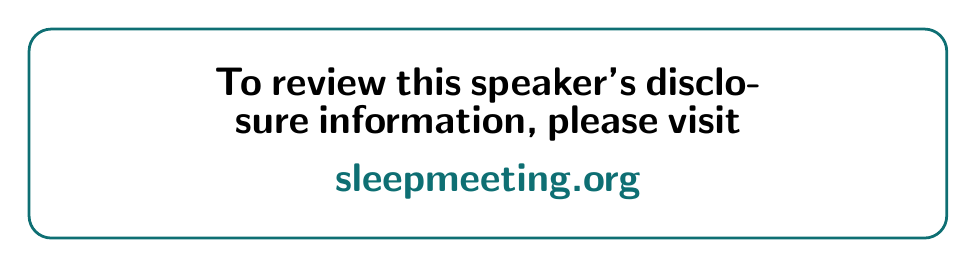
\begin{tikzpicture}
    \node[
      rounded corners=8pt,
      fill=white,
      draw=SleepTeal,
      line width=1.0pt,
      inner xsep=14pt,
      inner ysep=14pt,
      text width=0.88\linewidth,
      align=center
    ] {
      {\Large\bfseries To review this speaker's disclosure information, please visit}\\[0.25cm]
      {\Large\color{SleepTeal}\bfseries sleepmeeting.org}
    };
  \end{tikzpicture}
\end{frame}

\begin{frame}{SLEEP 2026 Photography Policy}
  \begin{columns}[T,totalwidth=\textwidth]
    \begin{column}{0.18\textwidth}
      \vspace{0.45cm}
      
\begin{tikzpicture}
        \node[circle,draw=SleepTeal,line width=1.2pt,minimum width=1.8cm] {\fontsize{24}{24}\selectfont\color{SleepTeal}\bfseries \checkmark};
      \end{tikzpicture}
    \end{column}
    \begin{column}{0.76\textwidth}
      \begin{itemize}
        \item Photography is permitted during this lecture unless a no-photography icon is shown.
        \item Photographs are allowed for personal, social, or non-commercial use.
        \item Attendees may not use flash photography or otherwise distract presenters or attendees.
      \end{itemize}
    \end{column}
  \end{columns}
\end{frame}

\begin{frame}{Wearables and Longitudinal Monitoring of Sleep and Circadian Traits}
  \begin{columns}[T,totalwidth=\textwidth]
    \begin{column}{0.48\textwidth}
      \begin{block}{Why this matters}
        \begin{itemize}
          \item Sleep is important to health and chronic disease risk.
          \item Most large epidemiologic studies rely on self-report or short-term monitoring.
          \item Wearables create scalable, repeated measurements of sleep timing, duration, and variability.
        \end{itemize}
      \end{block}
      \vspace{0.18cm}
      \vspace{-0.05cm}
      \takeaway{Longitudinal Fitbit data move sleep phenotyping from sparse recall to repeated behavioral measurement.}
    \end{column}
    \begin{column}{0.47\textwidth}
      \begin{block}{Published context}
        Prior All of Us Fitbit analyses have linked wearable-derived sleep measures to clinical phenotypes, motivating higher-resolution longitudinal modeling of sleep behavior.
      \end{block}
      \vspace{0.35cm}
      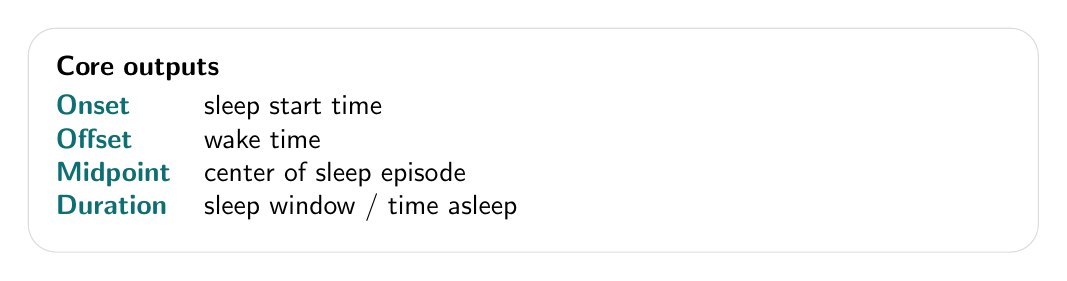
\begin{tikzpicture}
        \node[rounded corners=10pt,fill=white,draw=NightInk!15,inner sep=10pt,text width=\linewidth] {
          \textbf{Core outputs}\\[3pt]
          \begin{tabular}{@{}ll@{}}
            \textcolor{SleepTeal}{\bfseries Onset} & sleep start time\\
            \textcolor{SleepTeal}{\bfseries Offset} & wake time\\
            \textcolor{SleepTeal}{\bfseries Midpoint} & center of sleep episode\\
            \textcolor{SleepTeal}{\bfseries Duration} & sleep window / time asleep\\
          \end{tabular}
        };
      \end{tikzpicture}
    \end{column}
  \end{columns}
\end{frame}

\begin{frame}{Sources of Variability}
  \begin{columns}[T,totalwidth=\textwidth]
    \begin{column}{0.48\textwidth}
      \begin{block}{Extrinsic}
        \begin{itemize}
          \item Weekdays vs. weekends / free days
          \item Seasonality and holidays
          \item Environmental exposures: photoperiod, temperature, humidity, daylight saving time
        \end{itemize}
      \end{block}
    \end{column}
    \begin{column}{0.48\textwidth}
      \begin{block}{Intrinsic and social}
        \begin{itemize}
          \item Age and sex
          \item Employment status and social scheduling constraints
          \item Stable participant-level differences captured by repeated measures
        \end{itemize}
      \end{block}
    \end{column}
  \end{columns}
  \vspace{0.32cm}
  \takeaway{These factors are established individually, but longitudinal wearable data allow them to be modeled together within the same participants.}
\end{frame}

\begin{frame}{Study Aim}
  \vspace{0.5cm}
  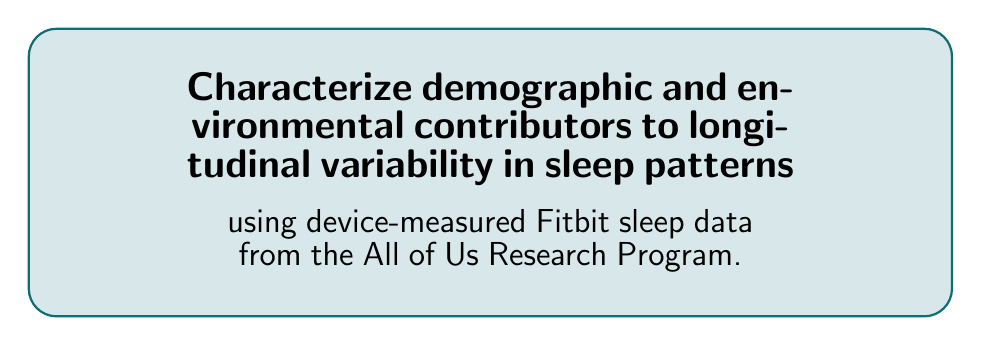
\begin{tikzpicture}
    \node[
      rounded corners=10pt,
      fill=SoftBlue,
      draw=SleepTeal,
      line width=0.8pt,
      inner xsep=15pt,
      inner ysep=16pt,
      text width=0.88\linewidth,
      align=center
    ] {
      {\Large\bfseries Characterize demographic and environmental contributors to longitudinal variability in sleep patterns}\\[0.28cm]
      {\large using device-measured Fitbit sleep data from the All of Us Research Program.}
    };
  \end{tikzpicture}
  \vspace{0.4cm}
  \begin{columns}[T,totalwidth=0.9\textwidth]
    \begin{column}{0.33\linewidth}\kpi{Onset}{sleep start}{SoftGold}\end{column}
    \begin{column}{0.33\linewidth}\kpi{Midpoint}{sleep timing}{SoftBlue}\end{column}
    \begin{column}{0.33\linewidth}\kpi{Duration}{sleep amount}{SoftGold}\end{column}
  \end{columns}
\end{frame}

\begin{frame}{All of Us Research Program and Fitbit Sleep}
  \begin{columns}[T,totalwidth=\textwidth]
    \begin{column}{0.46\textwidth}
      \begin{block}{All of Us}
        \begin{itemize}
          \item National longitudinal cohort with EHR, survey, genomic, and wearable data.
          \item Participant-level covariates include demographics, employment, BMI, ZIP3 geography, and socioeconomic context.
        \end{itemize}
      \end{block}
      \begin{block}{Fitbit measurements}
        \begin{itemize}
          \item Sleep daily summaries provide nightly sleep duration.
          \item Sleep-level records provide high-resolution onset/offset information.
          \item Repeated nights allow within-person modeling over age, season, and social schedule.
        \end{itemize}
      \end{block}
    \end{column}
    \begin{column}{0.50\textwidth}
      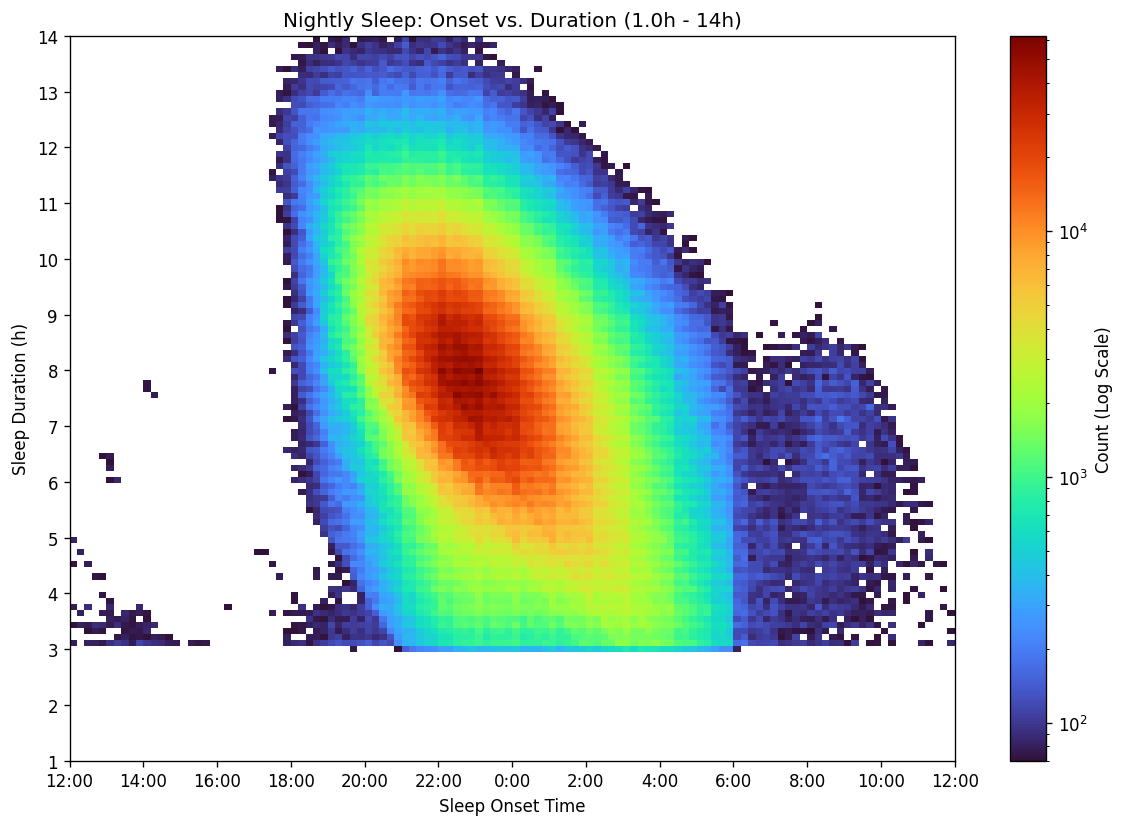
\includegraphics[width=\linewidth,height=0.70\textheight,keepaspectratio]{image36.png}\\[-2pt]
      \slidecite{Filtered person-night onset and duration density.}
    \end{column}
  \end{columns}
\end{frame}

\begin{frame}{Participant Characteristics}
  \begin{columns}[T,totalwidth=\textwidth]
    \begin{column}{0.42\textwidth}
      \begin{tabular}{@{}>{\raggedright\arraybackslash}p{0.66\linewidth}r@{}}
        \toprule
        Characteristic & Value\\
        \midrule
        Included participants & 42,290\\
        Filtered sleep nights & 22,428,610\\
        Age & 52 $\pm$ 17 y\\
        Female & 67.4\%\\
        Male & 32.3\%\\
        Nights recorded & 530 $\pm$ 730\\
        Nightly duration & 447 $\pm$ 65 min\\
        Nightly duration & 7.5 $\pm$ 1.1 h\\
        \bottomrule
      \end{tabular}
      \vspace{0.18cm}
      {\fontsize{7.3}{8.5}\selectfont
      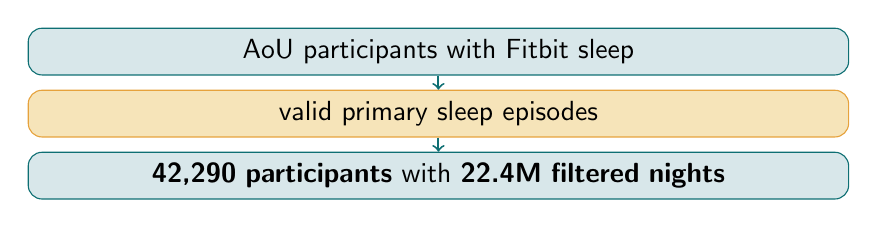
\begin{tikzpicture}[node distance=0.18cm]
        \node[rounded corners=5pt,fill=SoftBlue,draw=SleepTeal,align=center,text width=0.84\linewidth,inner ysep=4pt] (a) {AoU participants with Fitbit sleep};
        \node[rounded corners=5pt,fill=SoftGold,draw=WakeGold,align=center,text width=0.84\linewidth,inner ysep=4pt,below=of a] (b) {valid primary sleep episodes};
        \node[rounded corners=5pt,fill=SoftBlue,draw=SleepTeal,align=center,text width=0.84\linewidth,inner ysep=4pt,below=of b] (c) {\textbf{42,290 participants} with \textbf{22.4M filtered nights}};
        \draw[->,SleepTeal,line width=0.7pt] (a) -- (b);
        \draw[->,SleepTeal,line width=0.7pt] (b) -- (c);
      \end{tikzpicture}}
    \end{column}
    \begin{column}{0.55\textwidth}
      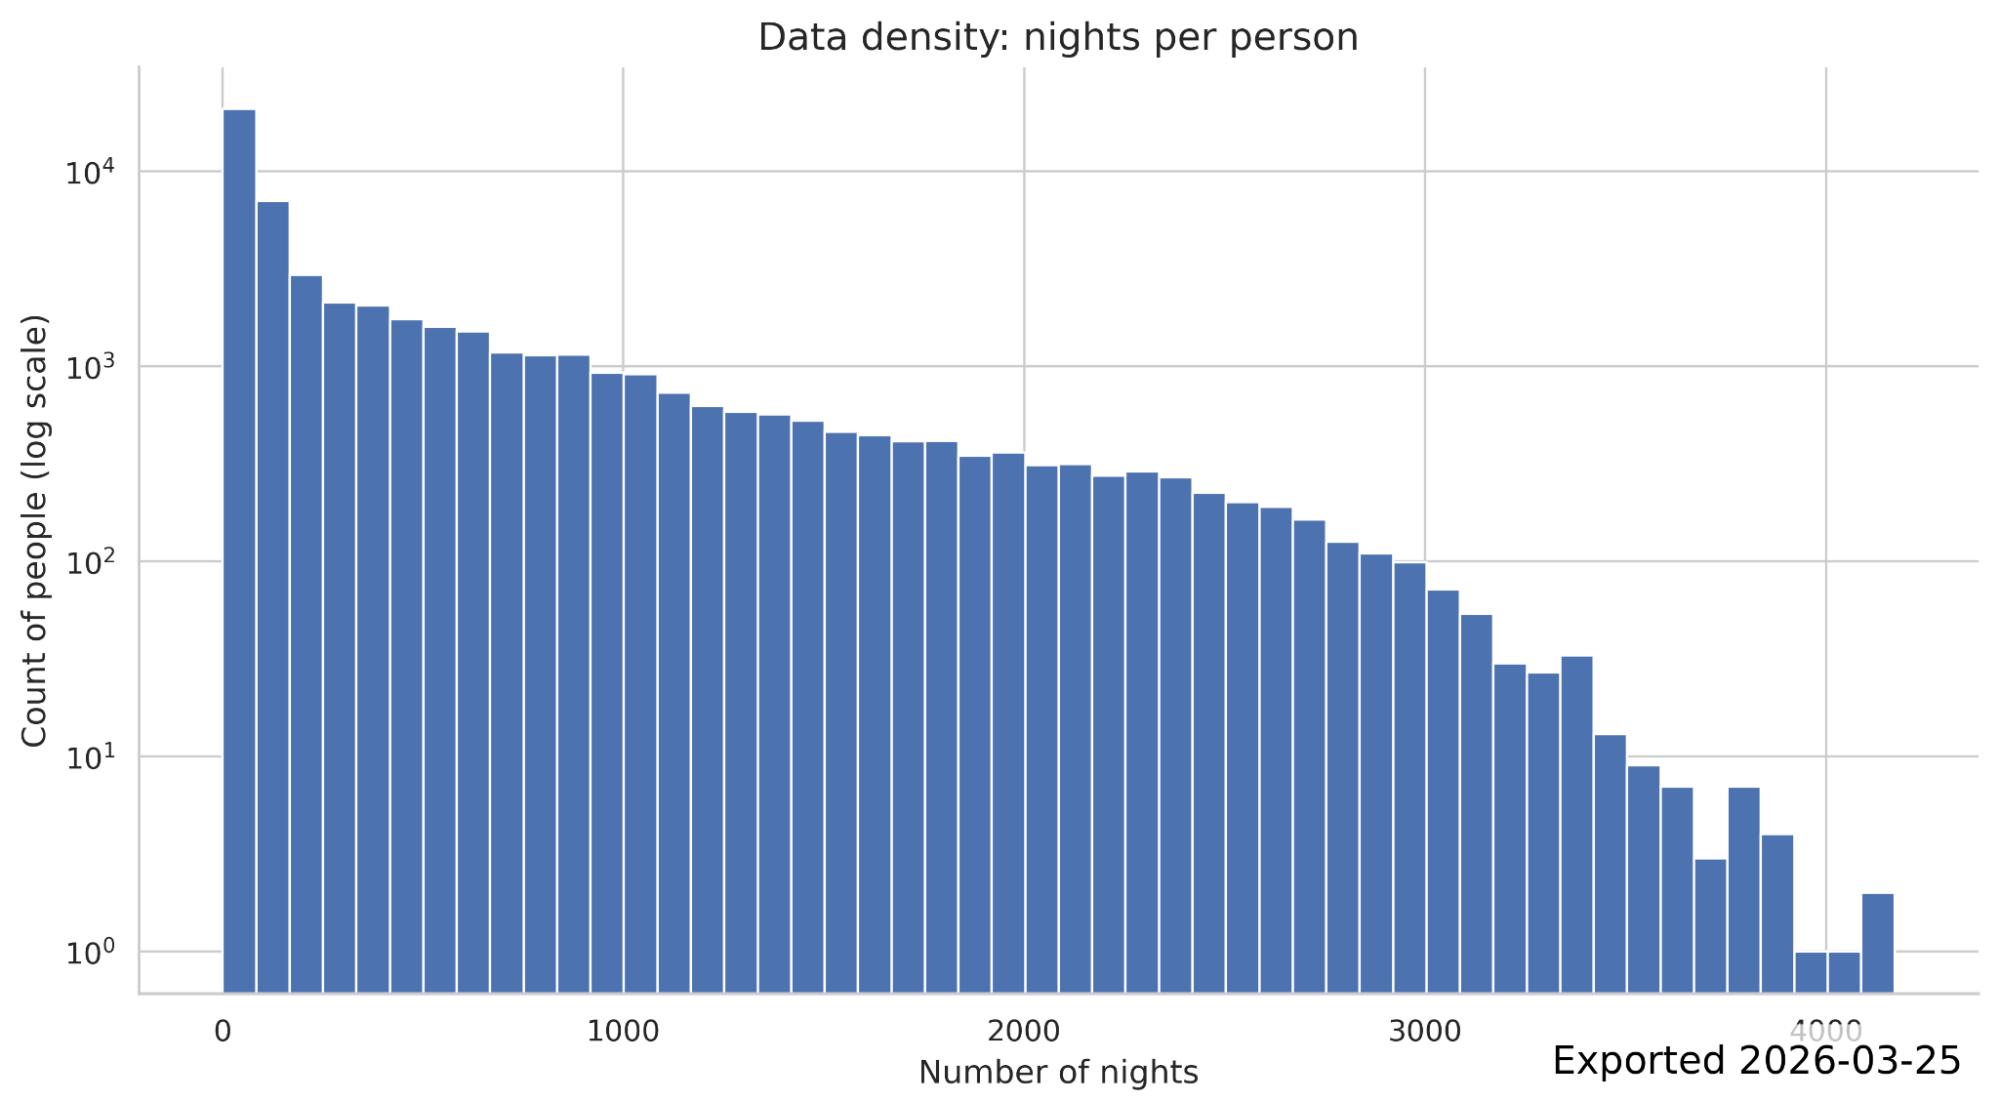
\includegraphics[width=\linewidth,height=0.74\textheight,keepaspectratio]{image37.png}\\[-2pt]
      \slidecite{Distribution of nights per participant.}
    \end{column}
  \end{columns}
\end{frame}

\begin{frame}{From Fitbit Records to Nightly Sleep Episodes}
  \begin{columns}[T,totalwidth=\textwidth]
    \begin{column}{0.46\textwidth}
      \begin{block}{Filtering and episode construction}
        \begin{itemize}
          \item Sleep-level records linked to daily summaries.
          \item Non-primary sleep excluded.
          \item Implausible raw durations excluded: $>18$h, zero/negative, common sensor artifact values.
          \item Segments clustered into nightly episodes; largest main sleep cluster retained per logical night.
          \item Sleep date assigned using a 6-hour backward shift.
        \end{itemize}
      \end{block}
    \end{column}
    \begin{column}{0.50\textwidth}
      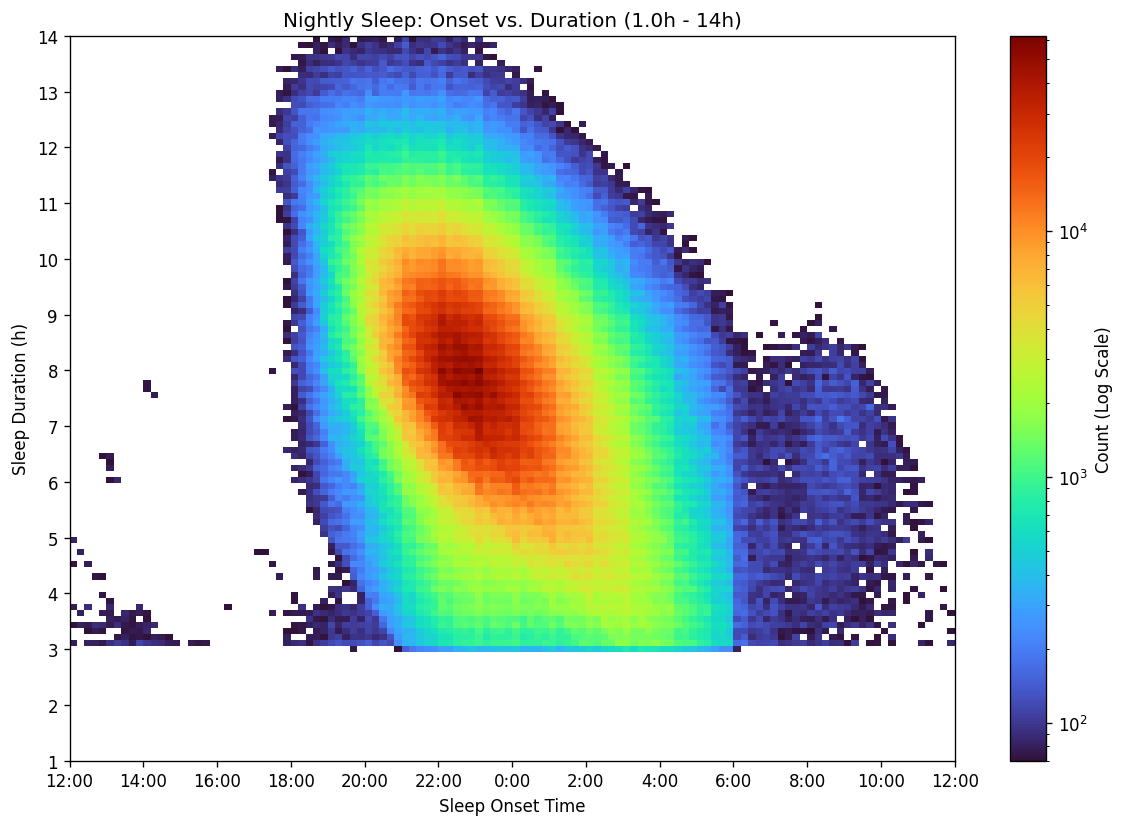
\includegraphics[width=\linewidth,height=0.72\textheight,keepaspectratio]{image36.png}\\[-2pt]
      \slidecite{Onset-duration density after filtering shows expected overnight sleep structure.}
    \end{column}
  \end{columns}
\end{frame}

\begin{frame}{Modeling Strategy}
  \begin{columns}[T,totalwidth=\textwidth]
    \begin{column}{0.53\textwidth}
      \begin{block}{Linear mixed-effects models}
        \[
          Y_{ij} \sim \mathrm{poly}(\mathrm{age}_{ij},2) + 
          \mathrm{weekend}_{ij} \times \mathrm{employment}_{i}
          + \mathrm{sex}_{i} + \mathrm{month}_{ij} + (1|\mathrm{person}_i)
        \]
      \end{block}
      \begin{itemize}
        \item Outcomes: onset, offset, midpoint, duration.
        \item Person random intercept controls stable between-person differences.
        \item Quadratic age captures non-linear lifespan trends.
        \item Employment-by-weekend interaction estimates social constraint/social jetlag patterns.
      \end{itemize}
    \end{column}
    \begin{column}{0.42\textwidth}
      \begin{block}{Time handling}
        \begin{itemize}
          \item Timing variables were linearized because distributions were primarily unimodal.
          \item Clock times before noon shifted forward by 24h.
          \item Example: 1:00 AM $\rightarrow$ 25.0; 11:00 PM $\rightarrow$ 23.0.
        \end{itemize}
      \end{block}
      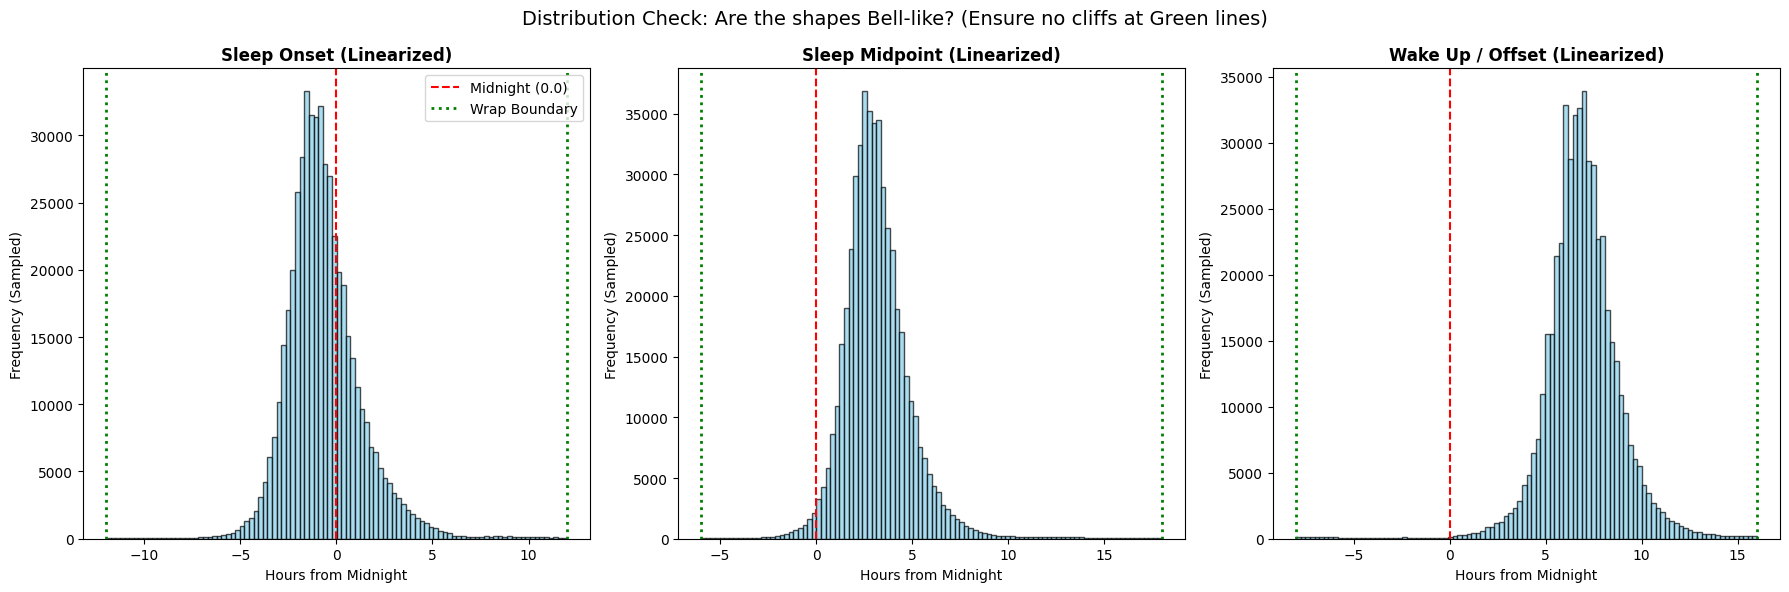
\includegraphics[width=\linewidth,height=0.31\textheight,keepaspectratio]{image9.png}
    \end{column}
  \end{columns}
\end{frame}

\begin{frame}{Sleep and Circadian Traits x Age and Sex}
  \begin{columns}[T,totalwidth=\textwidth]
    \begin{column}{0.36\textwidth}
      \begin{itemize}
        \item Age showed a quadratic association with sleep timing across the adult lifespan.
        \item Model-estimated sleep midpoint advanced by approximately 42 minutes from age 18 to age 57.
        \item Midpoint: 2:37 AM at age 18 vs. 1:54 AM at age 57.
      \end{itemize}
      \vspace{0.15cm}
      \takeaway{A simple linear age term would miss the lifespan shape of sleep timing.}
    \end{column}
    \begin{column}{0.61\textwidth}
      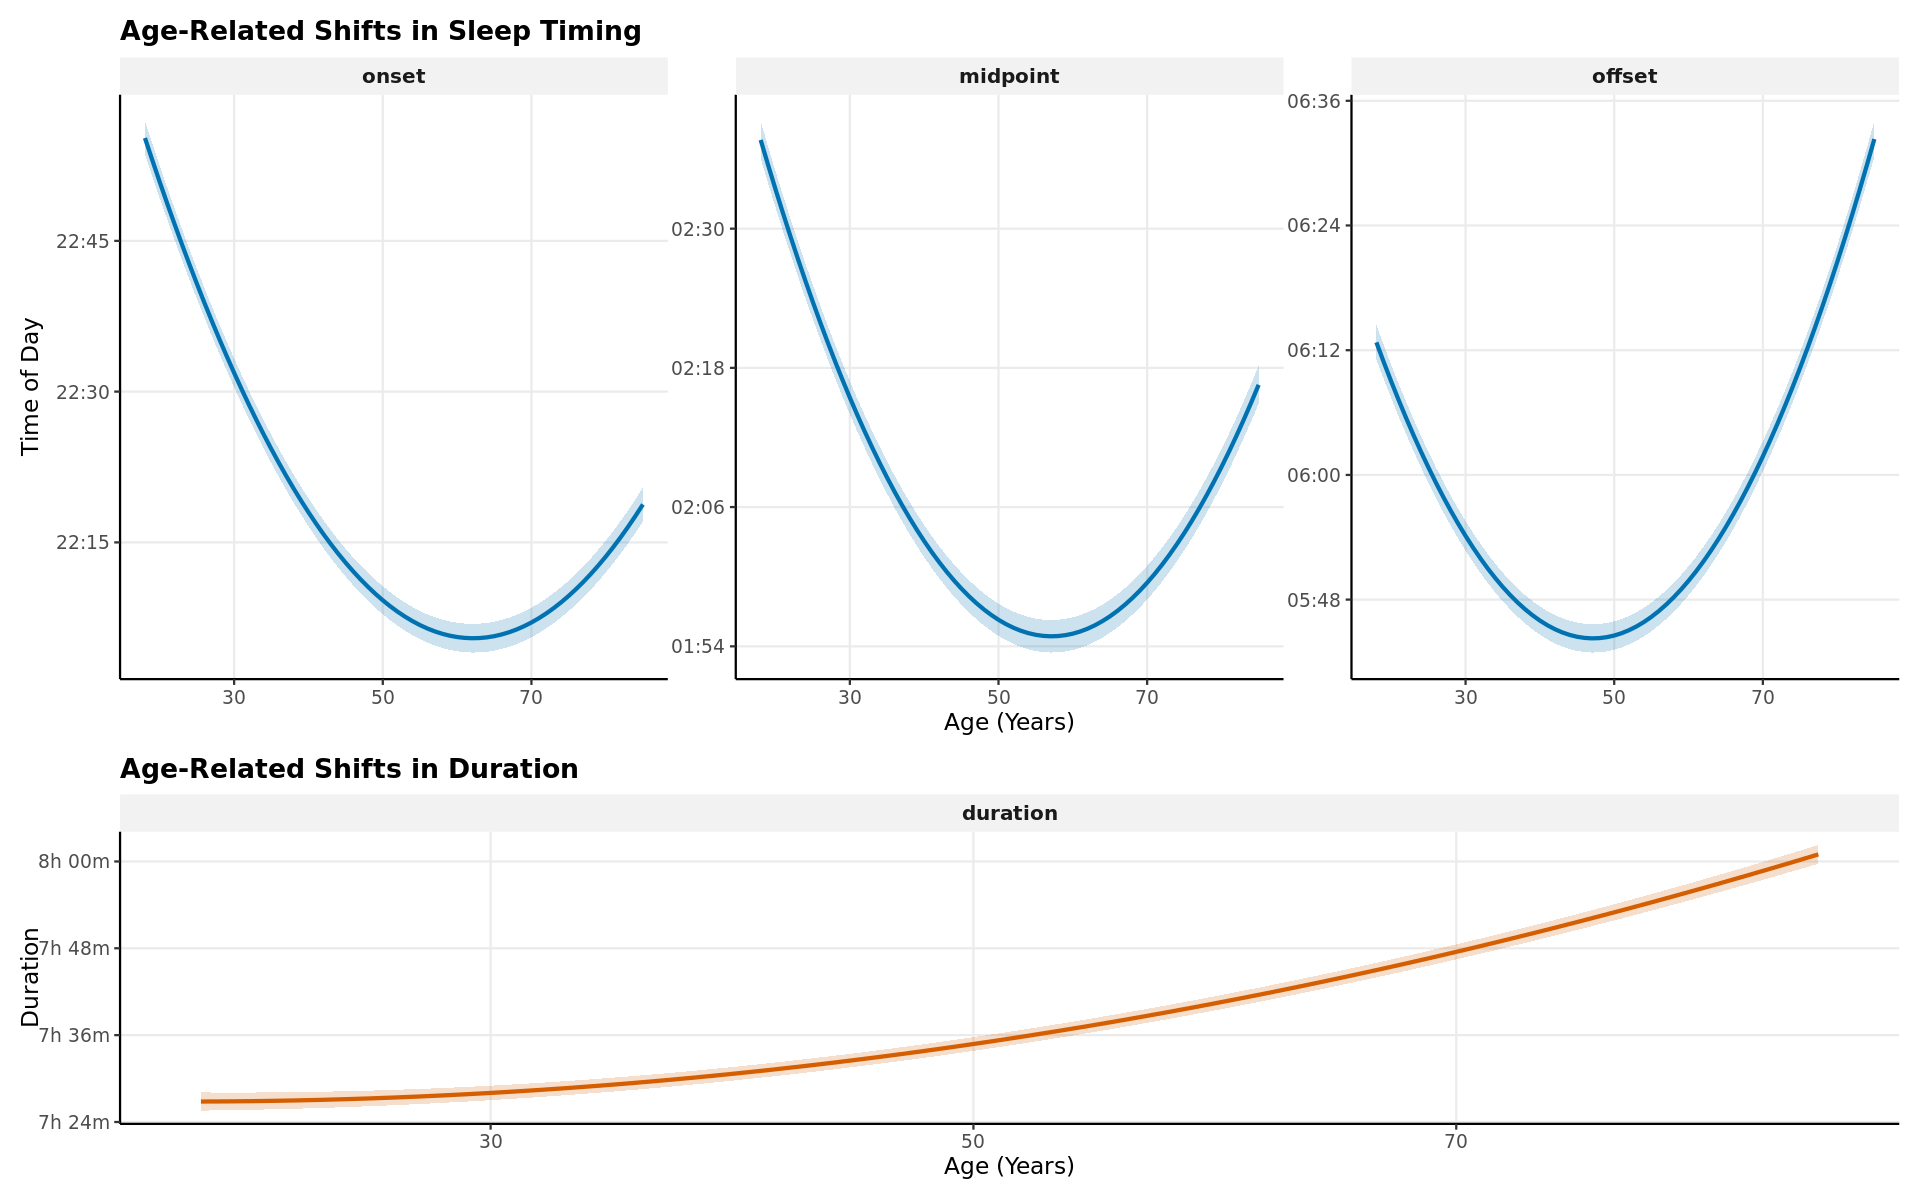
\includegraphics[width=\linewidth,height=0.76\textheight,keepaspectratio]{image14.png}
    \end{column}
  \end{columns}
\end{frame}

\begin{frame}{Sleep Duration Across the Adult Lifespan}
  \begin{columns}[T,totalwidth=\textwidth]
    \begin{column}{0.38\textwidth}
      \begin{itemize}
        \item Duration increased with age in adjusted models.
        \item Estimated gain: $>$34 minutes between ages 18 and 85.
        \item Age 18: 7.45h; age 85: 8.02h.
      \end{itemize}
      \vspace{0.15cm}
      \begin{block}{Why it matters}
        Timing and duration change together, so future analyses should consider mutually adjusted timing-duration phenotypes.
      \end{block}
    \end{column}
    \begin{column}{0.58\textwidth}
      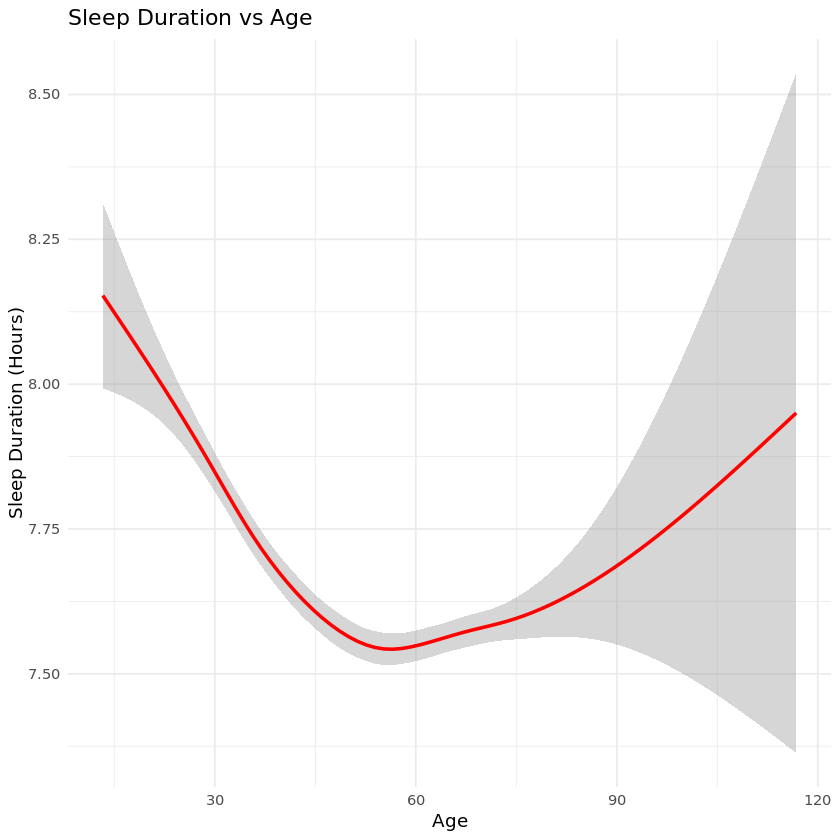
\includegraphics[width=\linewidth,height=0.73\textheight,keepaspectratio]{image46.png}
    \end{column}
  \end{columns}
\end{frame}

\begin{frame}{Sleep and Circadian Traits x Other Sociodemographics}
  \begin{columns}[T,totalwidth=\textwidth]
    \begin{column}{0.37\textwidth}
      \begin{itemize}
        \item Weekend status delayed midpoint, onset, and offset across employment groups.
        \item Participants employed for wages showed the largest midpoint delay.
        \item Employed for wages: weekday midpoint 3:26 AM vs. weekend midpoint 4:08 AM.
        \item Weekend sleep duration extended by approximately 28 minutes.
      \end{itemize}
      \vspace{0.12cm}
      \takeaway{Social timing constraints are visible in wearable sleep at population scale.}
    \end{column}
    \begin{column}{0.60\textwidth}
      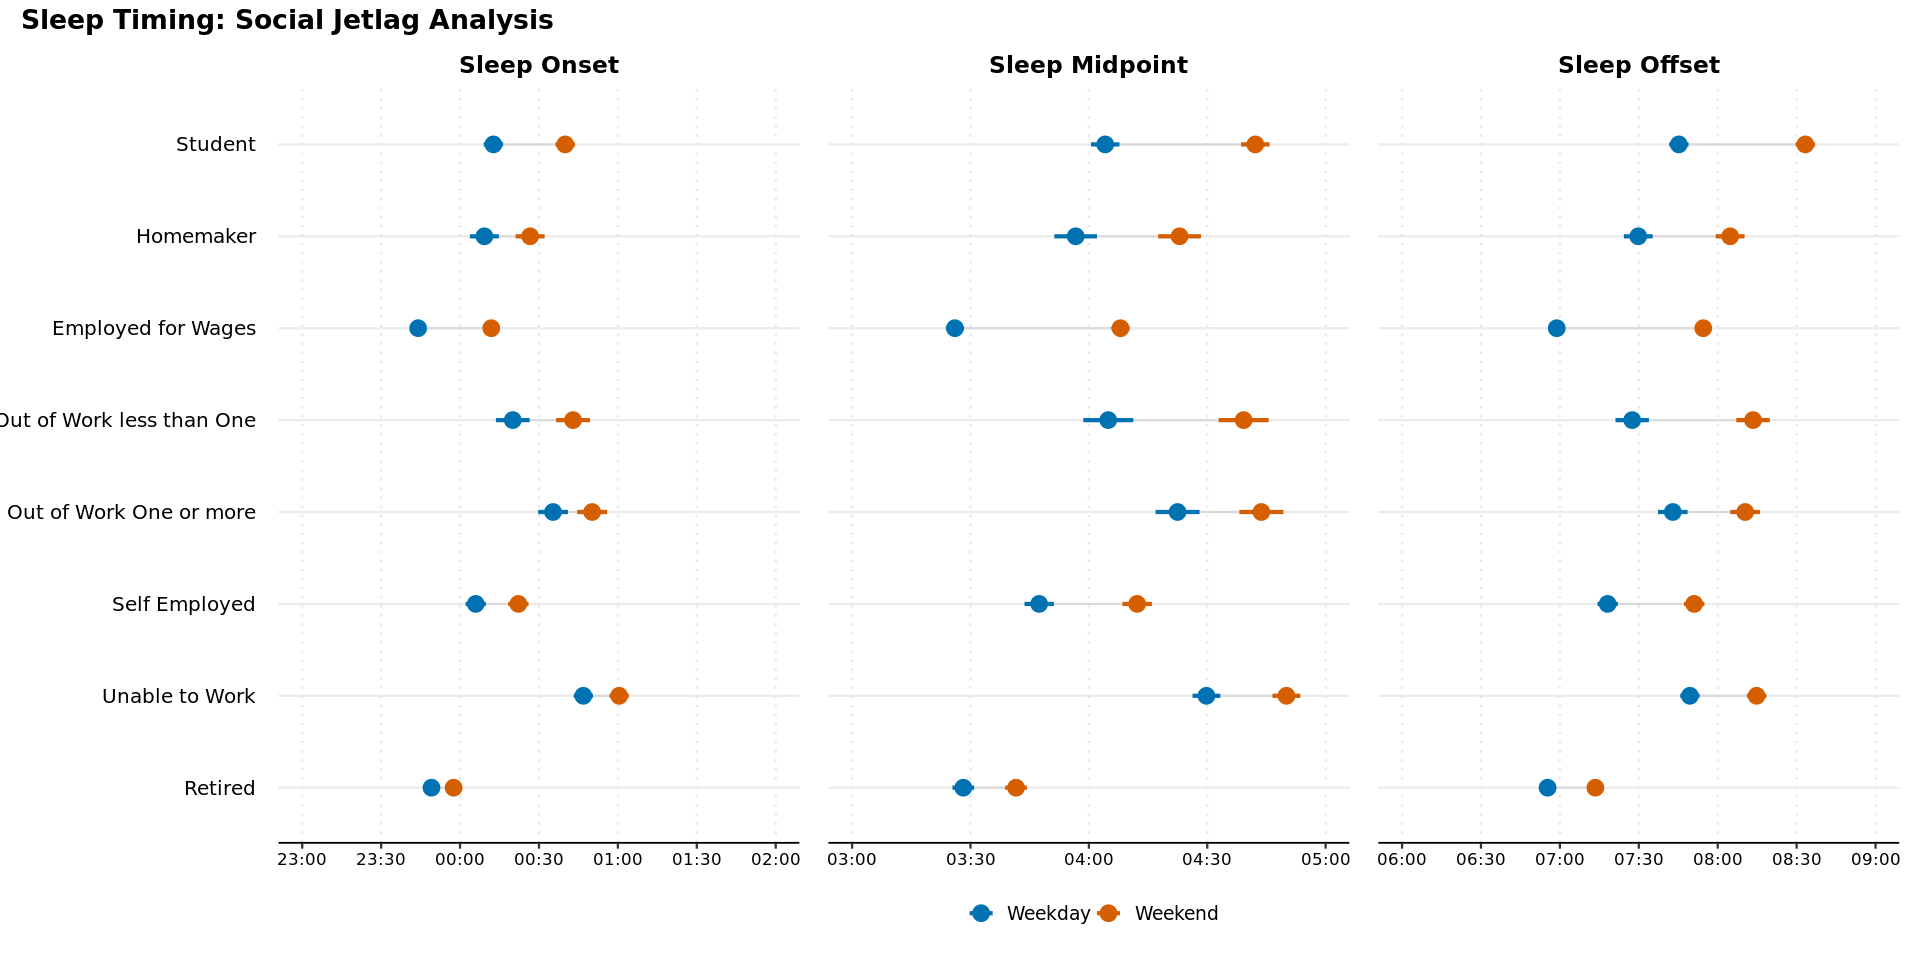
\includegraphics[width=\linewidth,height=0.76\textheight,keepaspectratio]{image22.png}
    \end{column}
  \end{columns}
\end{frame}

\begin{frame}{Sleep and Circadian Traits x Environmental Variables}
  \begin{columns}[T,totalwidth=\textwidth]
    \begin{column}{0.44\textwidth}
      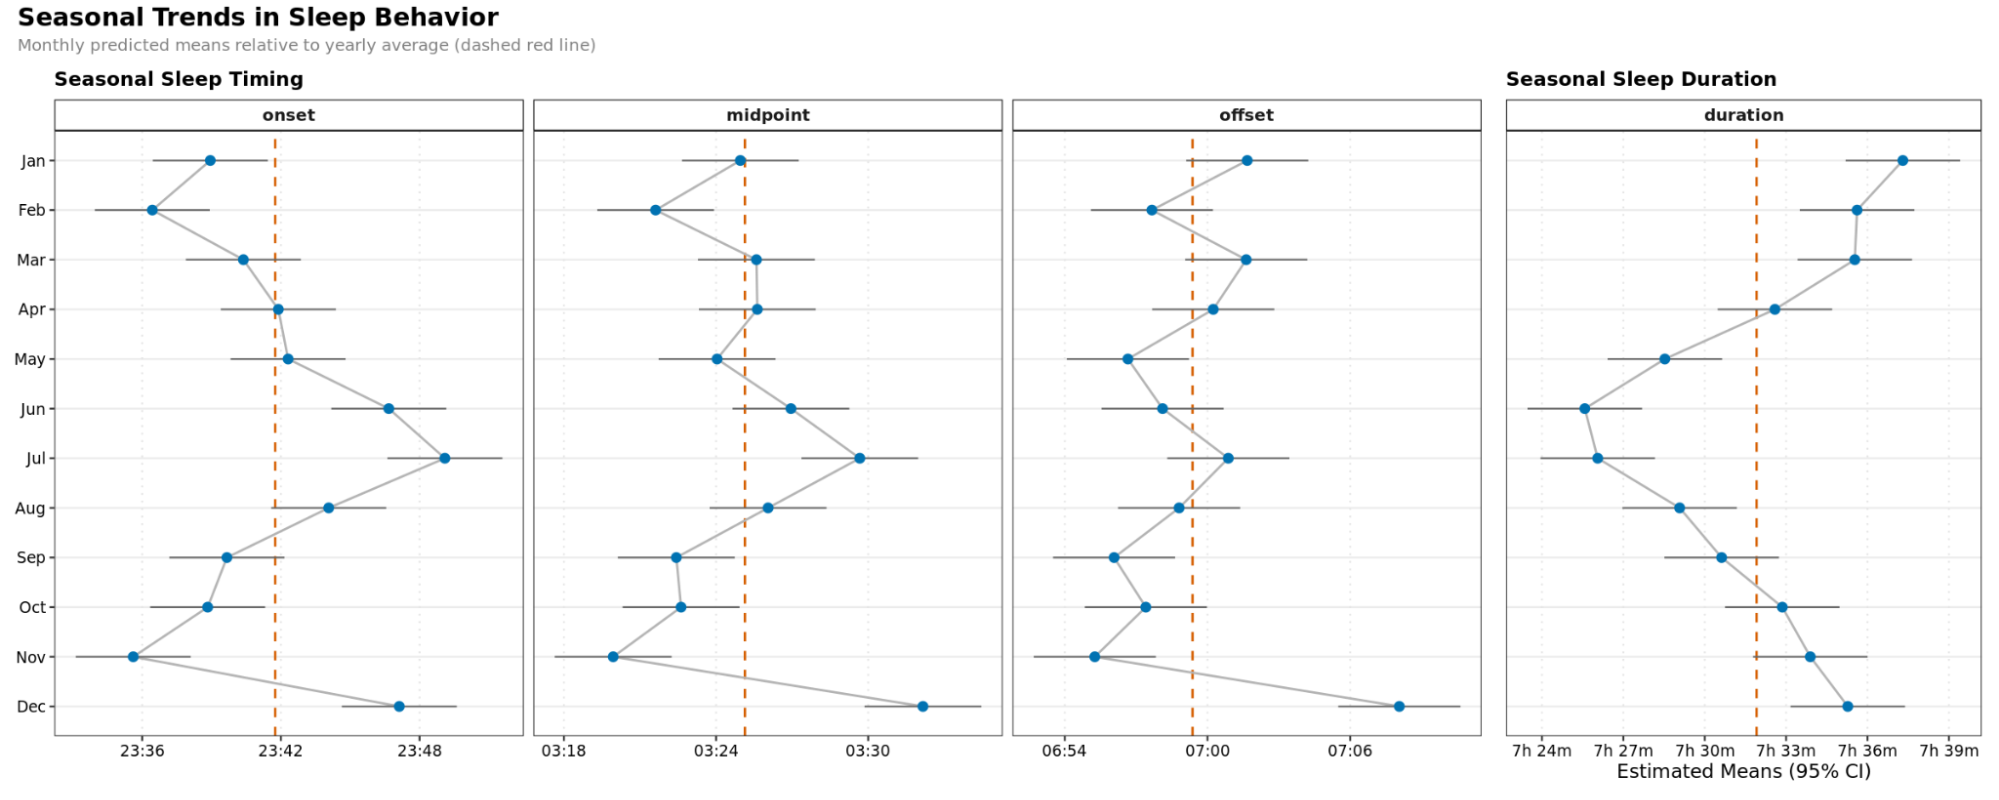
\includegraphics[width=\linewidth,height=0.64\textheight,keepaspectratio]{image21.png}
    \end{column}
    \begin{column}{0.52\textwidth}
      \begin{itemize}
        \item Month terms indicated seasonal differences in sleep behavior.
        \item Sleep duration was approximately 11 minutes lower in June than the January maximum.
        \item Unadjusted weekly trends suggest non-sinusoidal structure, likely mixing photoperiod, calendar behavior, holidays, and DST.
      \end{itemize}
      \vspace{0.18cm}
      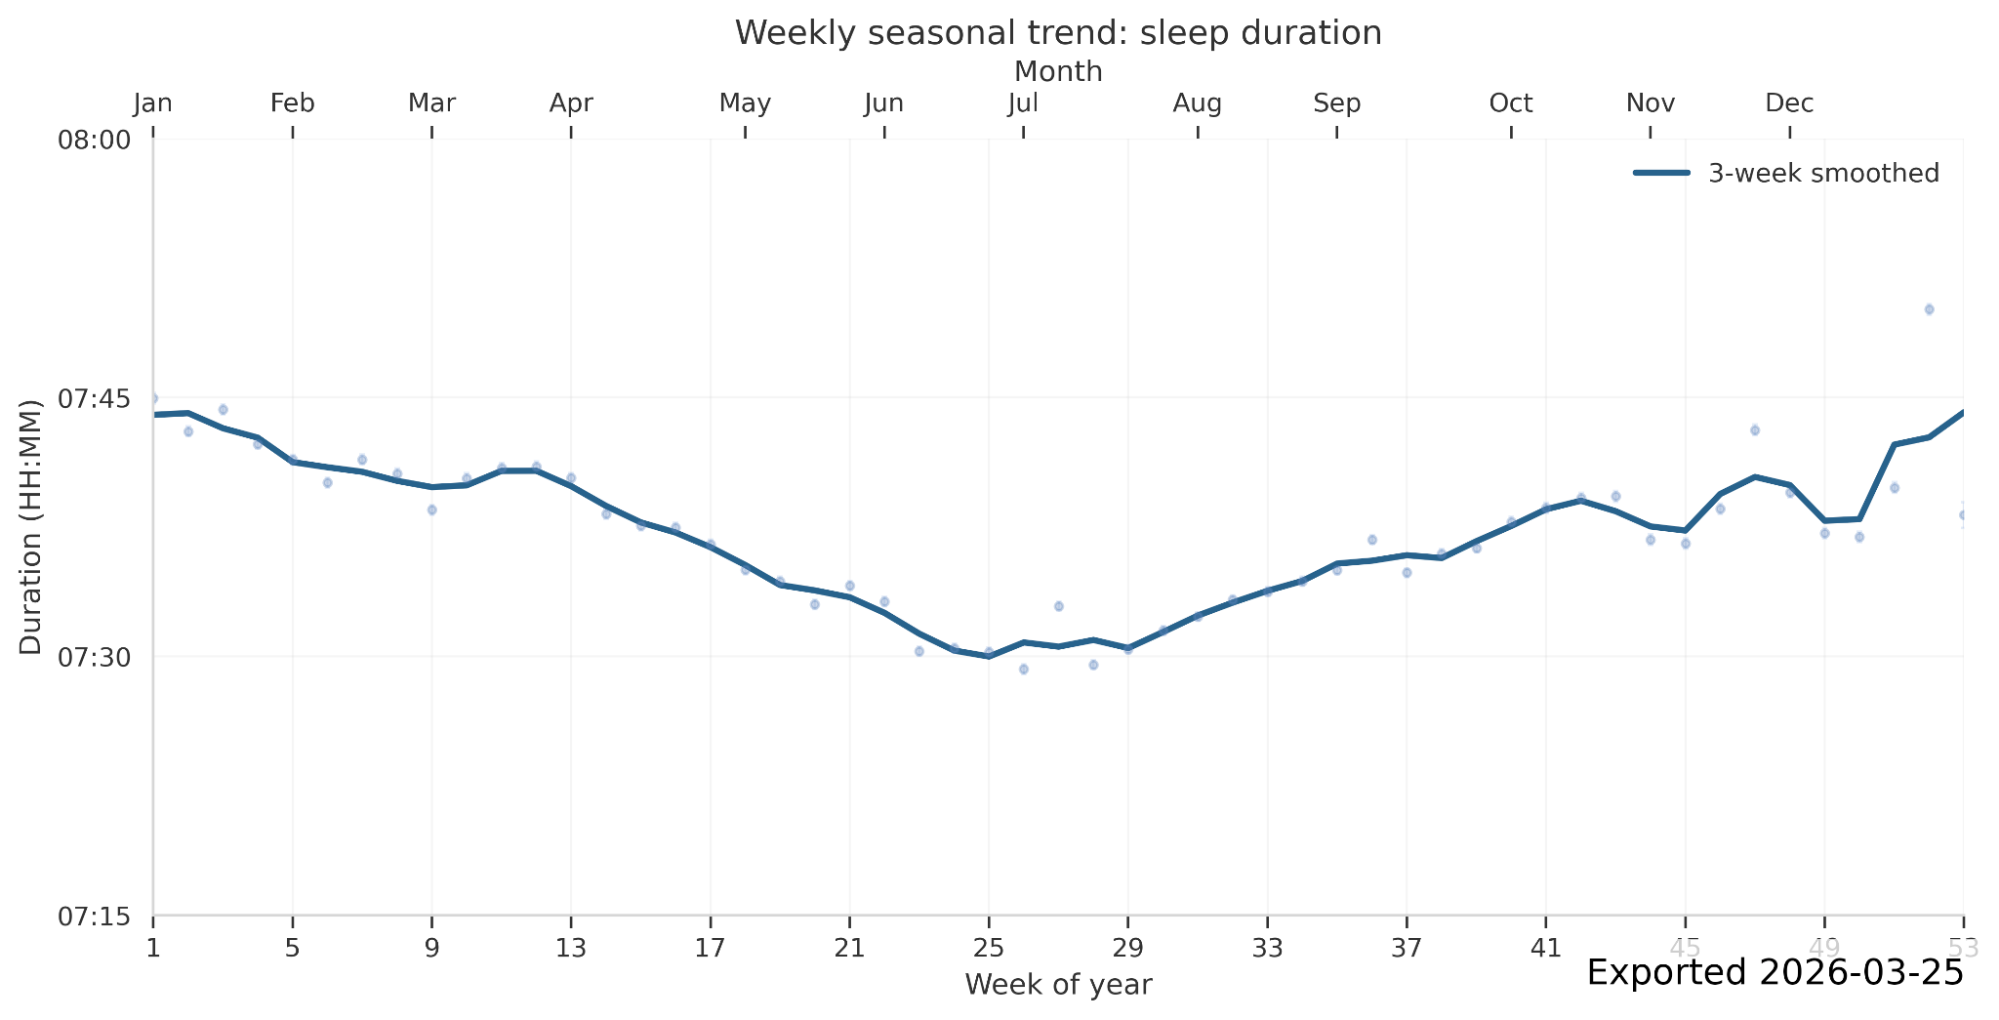
\includegraphics[width=\linewidth,height=0.34\textheight,keepaspectratio]{image52.png}
    \end{column}
  \end{columns}
\end{frame}

\begin{frame}{What This Adds}
  \begin{columns}[T,totalwidth=\textwidth]
    \begin{column}{0.48\textwidth}
      \begin{block}{Population-level characterization}
        \begin{itemize}
          \item Quantifies non-linear age effects in device-measured sleep.
          \item Separates workday/free-day structure from participant-level baselines.
          \item Provides adjusted estimates across employment categories.
        \end{itemize}
      \end{block}
    \end{column}
    \begin{column}{0.48\textwidth}
      \begin{block}{Foundation for next-stage analyses}
        \begin{itemize}
          \item Genetic studies of sleep timing and chronotype.
          \item Clinical risk stratification using longitudinal sleep phenotypes.
          \item Environmental extensions: photoperiod, temperature, humidity, DST.
        \end{itemize}
      \end{block}
    \end{column}
  \end{columns}
  \vspace{0.35cm}
  \takeaway{Large-scale wearable data can turn sleep timing from a sparse self-report phenotype into a longitudinal, model-ready exposure.}
\end{frame}

\begin{frame}{Limitations and Interpretation Guardrails}
  \begin{columns}[T,totalwidth=\textwidth]
    \begin{column}{0.48\textwidth}
      \begin{block}{Measurement}
        \begin{itemize}
          \item Fitbit-derived sleep depends on device classification of main sleep.
          \item Shift work is not directly measured; employment status is a proxy for social schedule constraints.
          \item Linearization works for the observed distribution but may under-represent true night-shift phenotypes.
        \end{itemize}
      \end{block}
    \end{column}
    \begin{column}{0.48\textwidth}
      \begin{block}{Cohort and covariates}
        \begin{itemize}
          \item AoU Fitbit participants are not a probability sample of U.S. adults.
          \item Pregnancy episode exclusion was not feasible in the V8 data context.
          \item ZIP3 geography is coarse for environmental and DST classification.
        \end{itemize}
      \end{block}
    \end{column}
  \end{columns}
\end{frame}

\begin{frame}{Conclusions and Future Directions}
  \begin{enumerate}
    \item Sleep timing and duration are dynamically structured by non-linear age effects.
    \item Employment and weekend status reveal strong social timing constraints, including measurable social jetlag.
    \item Seasonal patterns persist at population scale and motivate environmental modeling.
  \end{enumerate}
  \vspace{0.35cm}
  
\begin{tikzpicture}
    \node[
      rounded corners=9pt,
      fill=SleepTeal,
      text=white,
      inner xsep=12pt,
      inner ysep=10pt,
      text width=0.92\linewidth,
      align=center
    ] {\Large\bfseries Longitudinal wearable sleep data provide a scalable foundation for personalized circadian epidemiology.};
  \end{tikzpicture}
\end{frame}

\begin{frame}{Acknowledgements}
  \begin{columns}[T,totalwidth=\textwidth]
    \begin{column}{0.48\textwidth}
      \begin{block}{University of California, San Francisco}
        \begin{itemize}
          \item Mason Manetta
          \item Yue Leng, Ph.D.
          \item Shea Andrews, Ph.D.
        \end{itemize}
      \end{block}
      \begin{block}{Harvard Medical School / Brigham and Women's Hospital}
        \begin{itemize}
          \item Angus Burns, Ph.D.
        \end{itemize}
      \end{block}
    \end{column}
    \begin{column}{0.48\textwidth}
      \begin{block}{University of Kansas Medical Center}
        \begin{itemize}
          \item Diego R. Mazzotti, Ph.D.
        \end{itemize}
      \end{block}
      \begin{block}{Funding and support}
        \begin{itemize}
          \item All of Us Research Scholars Program
          \item RTI International All of Us Researcher Academy
          \item National Institutes of Health, Office of the Director
        \end{itemize}
      \end{block}
      \vspace{0.1cm}
      \takeaway{Questions and discussion}
    \end{column}
  \end{columns}
\end{frame}

\appendix

\begin{frame}{Backup: Validation Against Published AoU Sleep Structure}
  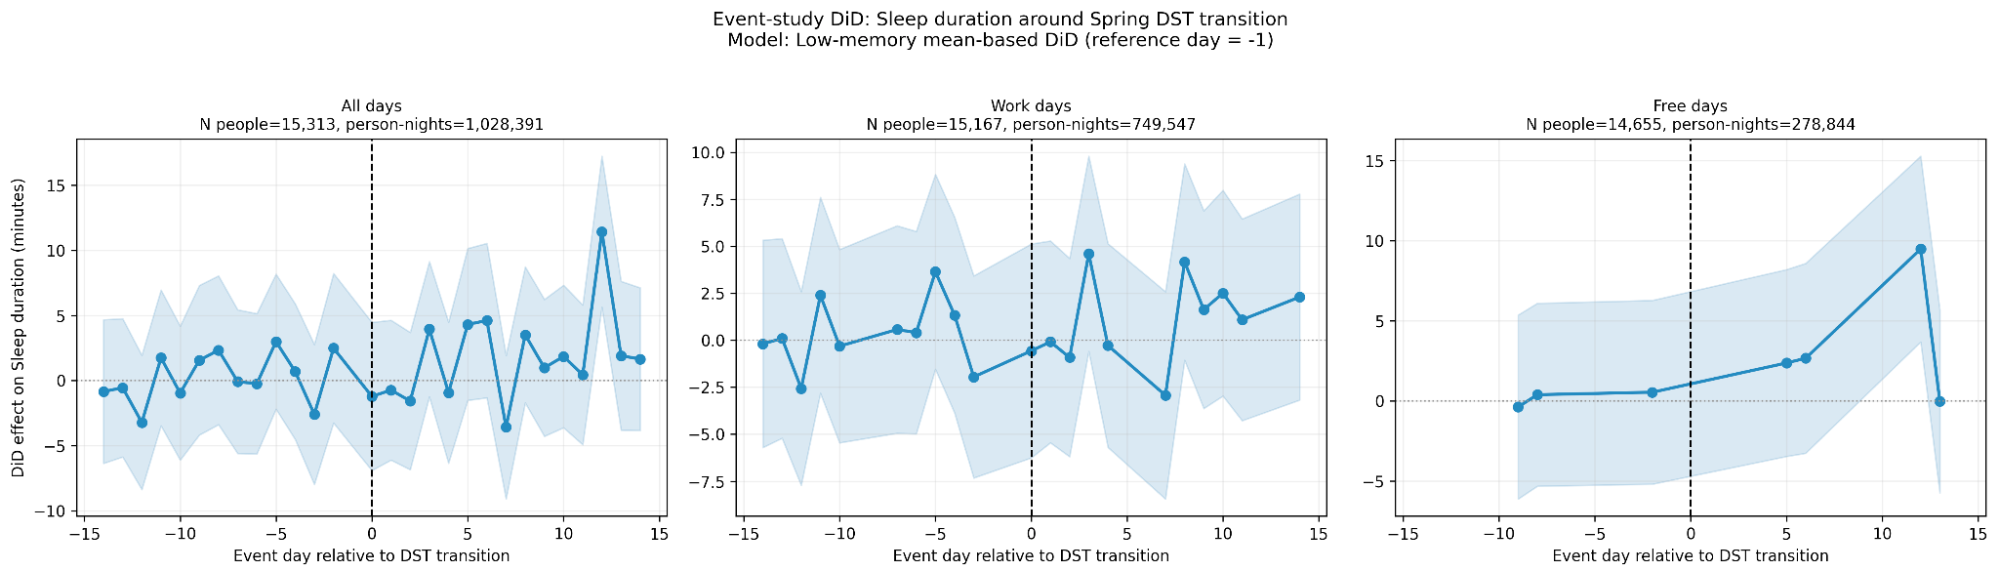
\includegraphics[width=\linewidth,height=0.78\textheight,keepaspectratio]{image23.png}
  \vspace{-0.05cm}
  \slidecite{Reference comparison with published All of Us Fitbit sleep structure; used during extraction validation.}
\end{frame}

\begin{frame}{Backup: Geographic and Environmental Extensions}
  \begin{columns}[T,totalwidth=\textwidth]
    \begin{column}{0.50\textwidth}
      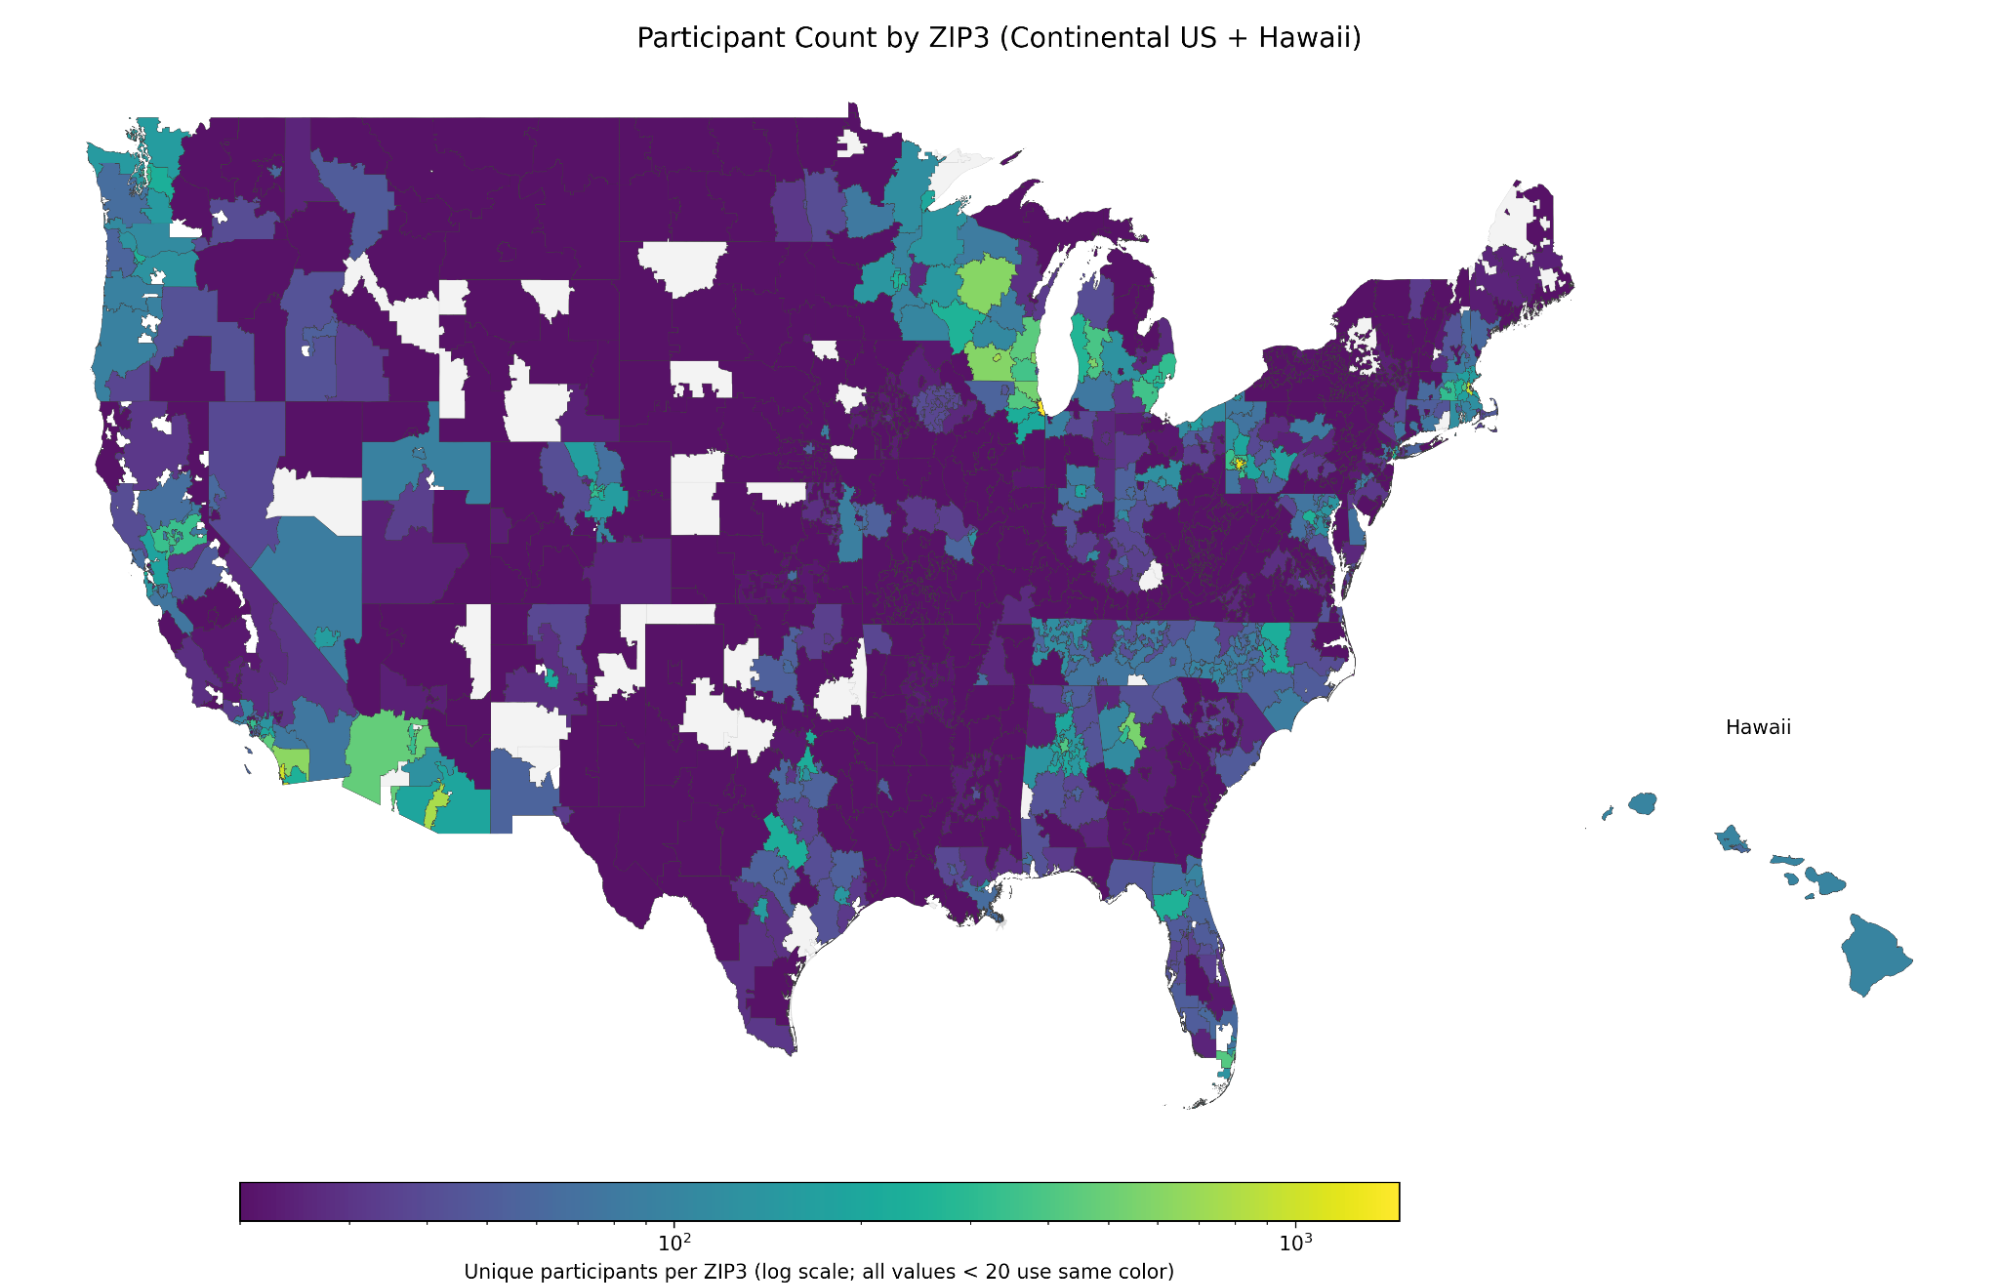
\includegraphics[width=\linewidth,height=0.68\textheight,keepaspectratio]{image39.png}\\[-2pt]
      \slidecite{Participant counts by ZIP3.}
    \end{column}
    \begin{column}{0.46\textwidth}
      \begin{itemize}
        \item ZIP3 enables coarse geography for SES, DST, photoperiod, and PRISM weather linkage.
        \item Future models can estimate temperature, vapor pressure deficit, precipitation, and photoperiod effects.
        \item Environmental analyses should account for ZIP3 population weighting and non-random participant geography.
      \end{itemize}
    \end{column}
  \end{columns}
\end{frame}

\begin{frame}{Backup: Daylight Saving Time Design}
  \begin{columns}[T,totalwidth=\textwidth]
    \begin{column}{0.48\textwidth}
      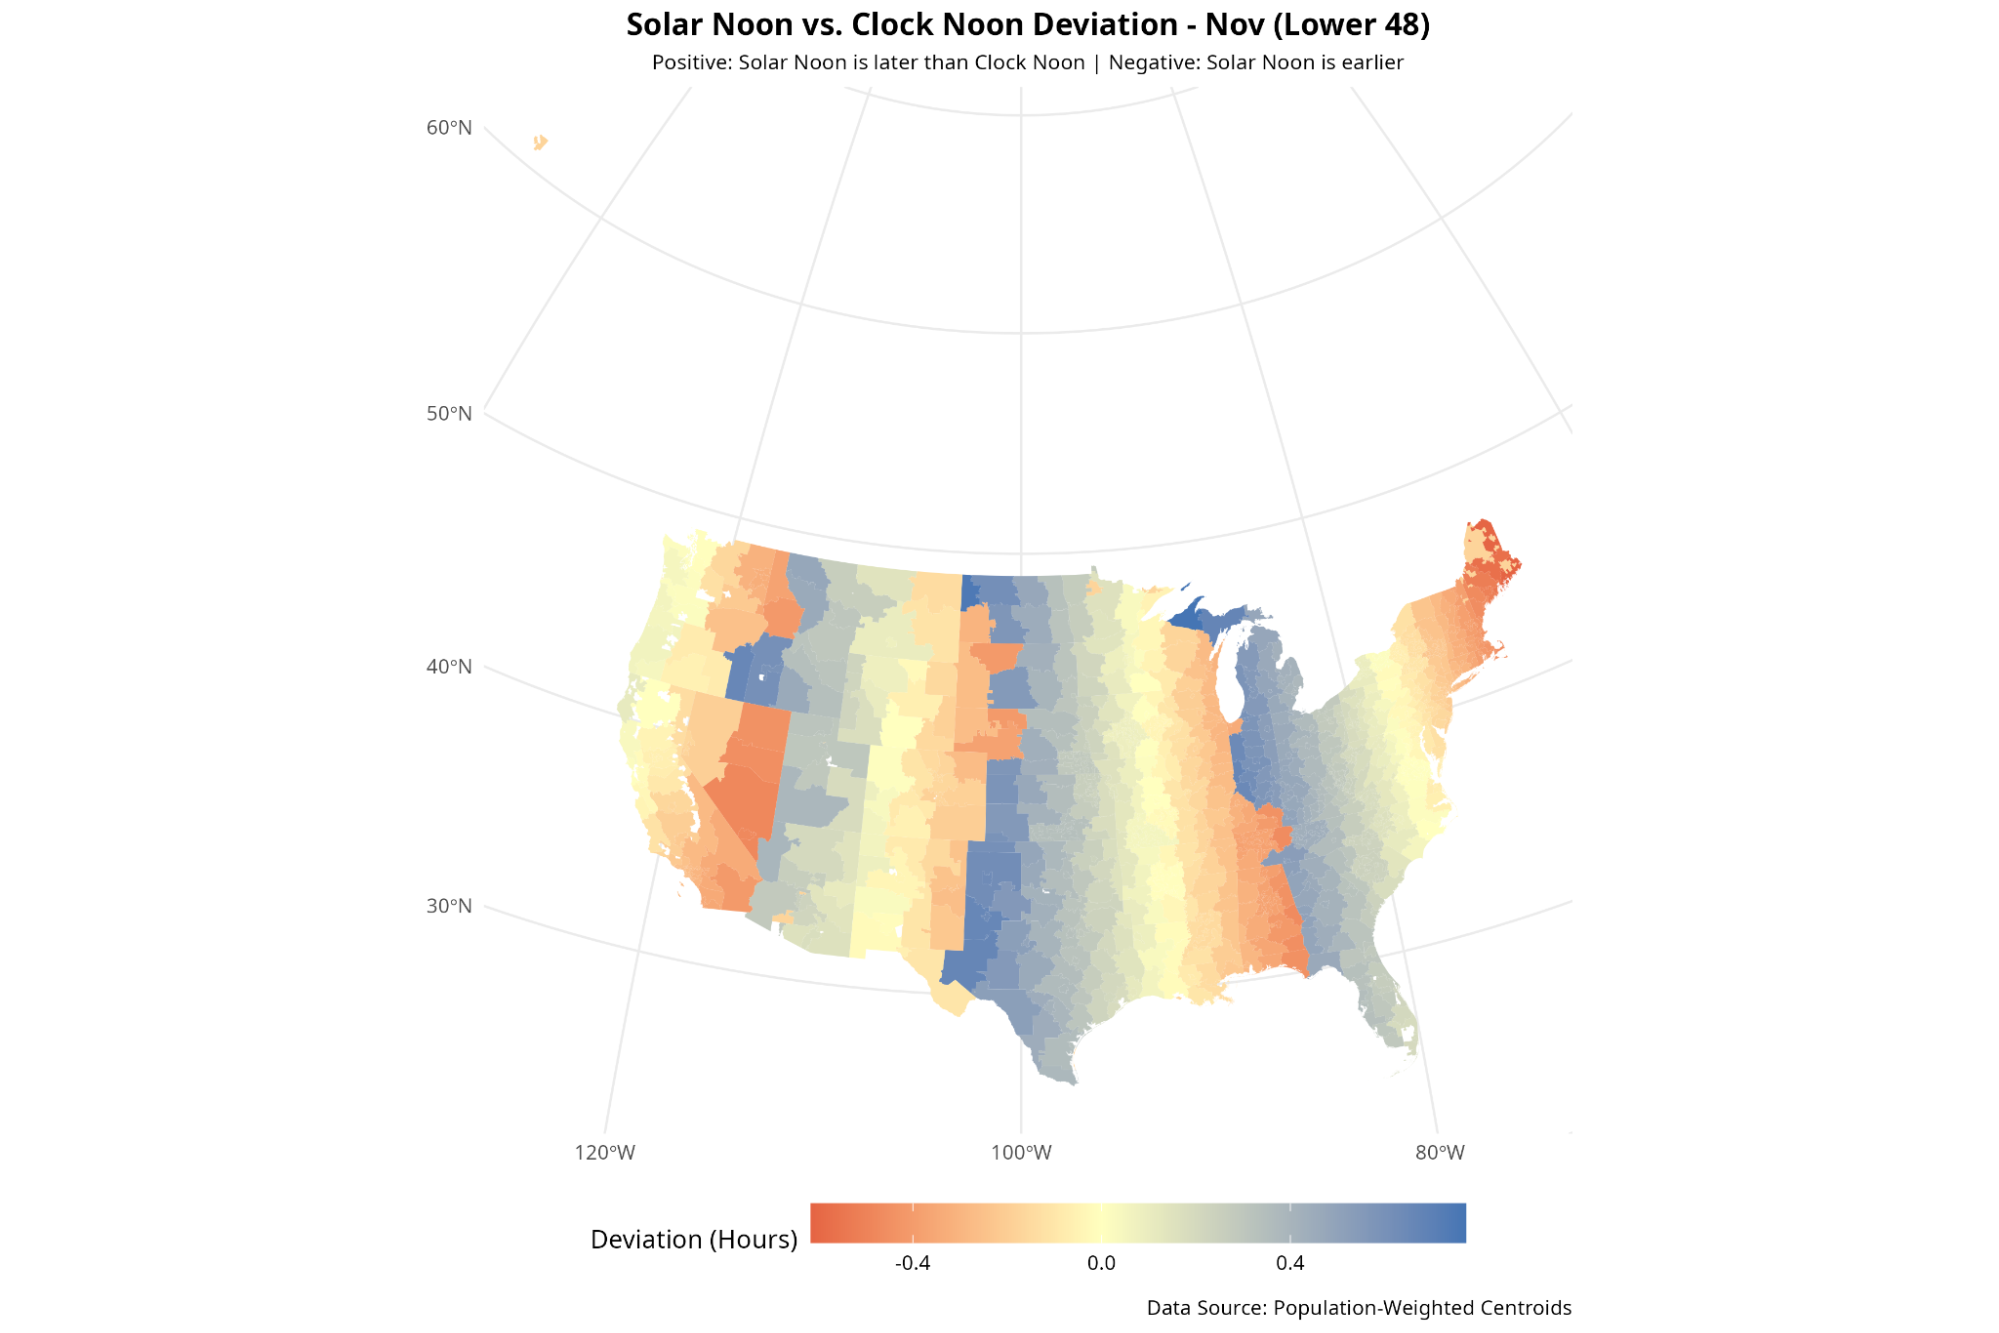
\includegraphics[width=\linewidth,height=0.62\textheight,keepaspectratio]{image42.png}
    \end{column}
    \begin{column}{0.48\textwidth}
      \begin{block}{DST contrast}
        \begin{itemize}
          \item Classify ZIP3 as DST-observing vs. non-DST control.
          \item Center each person-year using pre-transition baseline days -14 to -7.
          \item Estimate event-day differences around spring/fall transitions.
        \end{itemize}
      \end{block}
      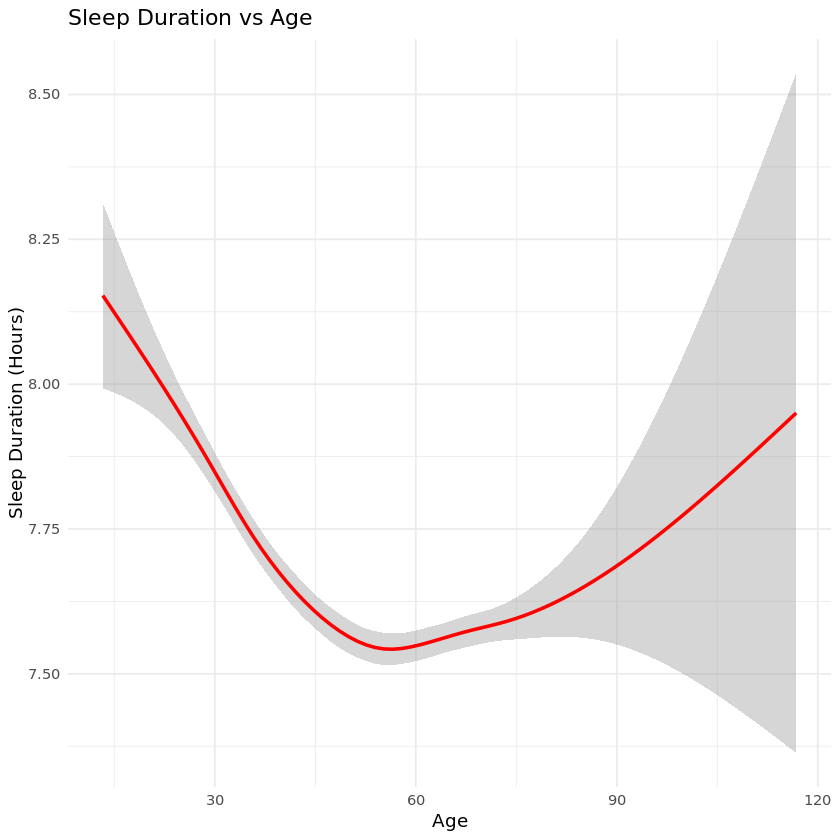
\includegraphics[width=\linewidth,height=0.28\textheight,keepaspectratio]{image46.png}
    \end{column}
  \end{columns}
\end{frame}

\end{document}
